\documentclass[a3paper,12pt]{extarticle} % Use extarticle for A3 paper size
\usepackage{graphicx} % Include this package for \includegraphics
\usepackage{amsmath}
\usepackage{amssymb} % Include this package for \mathbb
\usepackage[margin=1in]{geometry} % Adjust the margin as needed
\usepackage{float}
\usepackage{tikz} % Include this package for tikzpicture environment


\begin{document}

\author{kipngeno koech - bkoech}
\title{Homework 4 - Introduction to Probabilistic Graphical Models}   
\maketitle

\medskip

\maketitle

\section{Structure Learning}
\subsection{Tree-Selection and the Chow-Liu Algorithm}
Use the Chow-Liu Algorithm to learn the model (tree and parameters) that generated the following data.

\begin{figure}[H]
\centering
\includegraphics[width=0.8\textwidth]{q1.png}
\caption{The tree structure of the data.}
\label{fig:tree}
\end{figure}

The formula for calculating mutual information between the variables is:
\[
I(X;Y) = \sum_{x \in X} \sum_{y \in Y} p(x,y) \log\left(\frac{p(x,y)}{p(x)p(y)}\right)
\]
where \( p(x,y) \) is the joint probability of \( X \) and \( Y \), and \( p(x) \) and \( p(y) \) are the marginal probabilities of \( X \) and \( Y \), respectively.
The Chow-Liu algorithm is a method for constructing a maximum spanning tree (MST) from a set of variables based on their mutual information. The algorithm works as follows:
\begin{enumerate}
    \item Compute the mutual information \( I(X_i; X_j) \) for all pairs of variables \( (X_i, X_j) \).
    \item Create a weighted graph where each variable is a node and the edges are weighted by the mutual information values.
    \item Find the maximum spanning tree (MST) of the graph using Kruskal's or Prim's algorithm.
    \item The resulting tree structure represents the dependencies between the variables.
    \item Estimate the parameters of the tree structure using maximum likelihood estimation (MLE) or Bayesian methods.
    \item The resulting tree structure and parameters can be used for probabilistic inference and prediction.
\end{enumerate}
We need to compute the mutual information for all pairs of variables:
\begin{enumerate}
    \item \( I(X_1; X_2)\)
    \item \( I(X_1; X_3) \)
    \item \( I(X_2; X_3) \)
    \item \( I(X_1; X_4) \)
    \item \( I(X_2; X_4) \)
    \item \( I(X_3; X_4) \)
\end{enumerate}
\begin{enumerate}
    \item \( I(X_1; X_2) \)
let us start with the first one:
\begin{align*}
I(X_1; X_2) &= \sum_{x_1 \in X_1} \sum_{x_2 \in X_2} p(x_1,x_2) \log\left(\frac{p(x_1,x_2)}{p(x_1)p(x_2)}\right)\\
&= \sum_{x_1 \in X_1} \sum_{x_2 \in X_2} p(x_1,x_2) \log\left(\frac{p(x_1,x_2)}{p(x_1)p(x_2)}\right)\\
\end{align*}
so \(P(x_1, x_2)\) = (0,0), (0,1), (1,0), (1,1):
The mutual information is defined as:
\[
I(X_1; X_2) = \sum_{x_1 \in \{0,1\}} \sum_{x_2 \in \{0,1\}} P(x_1, x_2) \log_2 \left( \frac{P(x_1, x_2)}{P(x_1)P(x_2)} \right)
\]
Count the occurrences of each combination \((X_1 = x_1, X_2 = x_2)\):
\begin{itemize}
    \item \(X_1 = 0, X_2 = 0\): Occurs in 1 sample (row 8).
    \[
    P(X_1 = 0, X_2 = 0) = \frac{1}{9}
    \]
    \item \(X_1 = 0, X_2 = 1\): Occurs in 3 samples (rows 2, 5, 9).
    \[
    P(X_1 = 0, X_2 = 1) = \frac{3}{9} = \frac{1}{3}
    \]
    \item \(X_1 = 1, X_2 = 0\): Occurs in 2 samples (rows 1, 6).
    \[
    P(X_1 = 1, X_2 = 0) = \frac{2}{9}
    \]
    \item \(X_1 = 1, X_2 = 1\): Occurs in 3 samples (rows 3, 4, 7).
    \[
    P(X_1 = 1, X_2 = 1) = \frac{3}{9} = \frac{1}{3}
    \]
\end{itemize}
Verify: \(\frac{1}{9} + \frac{1}{3} + \frac{2}{9} + \frac{1}{3} = \frac{1 + 3 + 2 + 3}{9} = 1\).
Compute marginals:
\begin{itemize}
    \item For \(X_1\):
    \[
    P(X_1 = 0) = \frac{\text{4 samples (rows 2, 5, 8, 9)}}{9} = \frac{4}{9}, \quad P(X_1 = 1) = \frac{\text{5 samples (rows 1, 3, 4, 6, 7)}}{9} = \frac{5}{9}
    \]
    \item For \(X_2\):
    \[
    P(X_2 = 0) = \frac{\text{3 samples (rows 1, 6, 8)}}{9} = \frac{1}{3}, \quad P(X_2 = 1) = \frac{\text{6 samples (rows 2, 3, 4, 5, 7, 9)}}{9} = \frac{2}{3}
    \]
\end{itemize}

Computing the Mutual Information Terms\\
For each \((x_1, x_2)\), compute:
\[
P(x_1, x_2) \log_2 \left( \frac{P(x_1, x_2)}{P(x_1)P(x_2)} \right)
\]
\begin{itemize}
    \item \((x_1 = 0, x_2 = 0)\):
    \[
    P(X_1 = 0)P(X_2 = 0) = \frac{4}{9} \cdot \frac{1}{3} = \frac{4}{27}, \quad \frac{P(X_1 = 0, X_2 = 0)}{P(X_1 = 0)P(X_2 = 0)} = \frac{1/9}{4/27} = \frac{3}{4}
    \]
    \[
    \log_2 \left( \frac{3}{4} \right) \approx -0.415, \quad \text{Term} = \frac{1}{9} \cdot (-0.415) \approx -0.046
    \]
    \item \((x_1 = 0, x_2 = 1)\):
    \[
    P(X_1 = 0)P(X_2 = 1) = \frac{4}{9} \cdot \frac{2}{3} = \frac{8}{27}, \quad \frac{P(X_1 = 0, X_2 = 1)}{P(X_1 = 0)P(X_2 = 1)} = \frac{1/3}{8/27} = \frac{9}{8}
    \]
    \[
    \log_2 \left( \frac{9}{8} \right) \approx 0.170, \quad \text{Term} = \frac{1}{3} \cdot 0.170 \approx 0.057
    \]
    \item \((x_1 = 1, x_2 = 0)\):
    \[
    P(X_1 = 1)P(X_2 = 0) = \frac{5}{9} \cdot \frac{1}{3} = \frac{5}{27}, \quad \frac{P(X_1 = 1, X_2 = 0)}{P(X_1 = 1)P(X_2 = 0)} = \frac{2/9}{5/27} = \frac{6}{5}
    \]
    \[
    \log_2 \left( \frac{6}{5} \right) \approx 0.263, \quad \text{Term} = \frac{2}{9} \cdot 0.263 \approx 0.058
    \]
    \item \((x_1 = 1, x_2 = 1)\):
    \[
    P(X_1 = 1)P(X_2 = 1) = \frac{5}{9} \cdot \frac{2}{3} = \frac{10}{27}, \quad \frac{P(X_1 = 1, X_2 = 1)}{P(X_1 = 1)P(X_2 = 1)} = \frac{1/3}{10/27} = \frac{9}{10}
    \]
    \[
    \log_2 \left( \frac{9}{10} \right) \approx -0.152, \quad \text{Term} = \frac{1}{3} \cdot (-0.152) \approx -0.051
    \]
\end{itemize}

Sum the Terms:\\
Compute the mutual information:
\[
I(X_1; X_2) = (-0.046) + 0.057 + 0.058 - 0.051 \approx 0.018
\]

Thus, the mutual information is:
\[
I(X_1; X_2) \approx 0.018 \text{ bits}
\]

This value represents the weight of the edge between \(X_1\) and \(X_2\) in the Chow-Liu algorithm's graph.
\item \(X_1; X_3\):
\begin{align}
I(X_1; X_3) &= \sum_{x_1 \in X_1} \sum_{x_3 \in X_3} p(x_1,x_3) \log\left(\frac{p(x_1,x_3)}{p(x_1)p(x_3)}\right)\\
&= \sum_{x_1 \in X_1} \sum_{x_3 \in X_3} p(x_1,x_3) \log\left(\frac{p(x_1,x_3)}{p(x_1)p(x_3)}\right)\\
\end{align}
Given a dataset with 9 samples and 4 binary variables (\(X_1, X_2, X_3, X_4\)), we compute the mutual information \(I(X_1; X_3)\) for the Chow-Liu algorithm.

The mutual information is:
\[
I(X_1; X_3) = \sum_{x_1 \in \{0,1\}} \sum_{x_3 \in \{0,1\}} P(x_1, x_3) \log_2 \left( \frac{P(x_1, x_3)}{P(x_1)P(x_3)} \right)
\]

\textbf{Compute Joint Probabilities}: Count occurrences of \((X_1 = x_1, X_3 = x_3)\):
\begin{itemize}
    \item \(X_1 = 0, X_3 = 0\): 3 samples (rows 2, 5, 9).
    \[
    P(X_1 = 0, X_3 = 0) = \frac{3}{9} = \frac{1}{3}
    \]
    \item \(X_1 = 0, X_3 = 1\): 1 sample (row 8).
    \[
    P(X_1 = 0, X_3 = 1) = \frac{1}{9}
    \]
    \item \(X_1 = 1, X_3 = 0\): 4 samples (rows 1, 3, 6, 7).
    \[
    P(X_1 = 1, X_3 = 0) = \frac{4}{9}
    \]
    \item \(X_1 = 1, X_3 = 1\): 1 sample (row 4).
    \[
    P(X_1 = 1, X_3 = 1) = \frac{1}{9}
    \]
\end{itemize}
Verify: \(\frac{1}{3} + \frac{1}{9} + \frac{4}{9} + \frac{1}{9} = \frac{3 + 1 + 4 + 1}{9} = 1\).

\textbf{Compute Marginal Probabilities}:
\begin{itemize}
    \item \(X_1\):
    \[
    P(X_1 = 0) = \frac{\text{4 samples (rows 2, 5, 8, 9)}}{9} = \frac{4}{9}, \quad P(X_1 = 1) = \frac{\text{5 samples (rows 1, 3, 4, 6, 7)}}{9} = \frac{5}{9}
    \]
    \item \(X_3\):
    \[
    P(X_3 = 0) = \frac{\text{7 samples (rows 1, 2, 3, 5, 6, 7, 9)}}{9} = \frac{7}{9}, \quad P(X_3 = 1) = \frac{\text{2 samples (rows 4, 8)}}{9} = \frac{2}{9}
    \]
\end{itemize}

\textbf{Compute Mutual Information Terms}:
For each \((x_1, x_3)\), compute \(P(x_1, x_3) \log_2 \left( \frac{P(x_1, x_3)}{P(x_1)P(x_3)} \right)\):
\begin{itemize}
    \item \((x_1 = 0, x_3 = 0)\):
    \[
    P(X_1 = 0)P(X_3 = 0) = \frac{4}{9} \cdot \frac{7}{9} = \frac{28}{81}, \quad \frac{P(X_1 = 0, X_3 = 0)}{P(X_1 = 0)P(X_3 = 0)} = \frac{1/3}{28/81} = \frac{27}{28}
    \]
    \[
    \log_2 \left( \frac{27}{28} \right) \approx -0.053, \quad \text{Term} = \frac{1}{3} \cdot (-0.053) \approx -0.018
    \]
    \item \((x_1 = 0, x_3 = 1)\):
    \[
    P(X_1 = 0)P(X_3 = 1) = \frac{4}{9} \cdot \frac{2}{9} = \frac{8}{81}, \quad \frac{P(X_1 = 0, X_3 = 1)}{P(X_1 = 0)P(X_3 = 1)} = \frac{1/9}{8/81} = \frac{9}{8}
    \]
    \[
    \log_2 \left( \frac{9}{8} \right) \approx 0.170, \quad \text{Term} = \frac{1}{9} \cdot 0.170 \approx 0.019
    \]
    \item \((x_1 = 1, x_3 = 0)\):
    \[
    P(X_1 = 1)P(X_3 = 0) = \frac{5}{9} \cdot \frac{7}{9} = \frac{35}{81}, \quad \frac{P(X_1 = 1, X_3 = 0)}{P(X_1 = 1)P(X_3 = 0)} = \frac{4/9}{35/81} = \frac{36}{35}
    \]
    \[
    \log_2 \left( \frac{36}{35} \right) \approx 0.042, \quad \text{Term} = \frac{4}{9} \cdot 0.042 \approx 0.019
    \]
    \item \((x_1 = 1, x_3 = 1)\):
    \[
    P(X_1 = 1)P(X_3 = 1) = \frac{5}{9} \cdot \frac{2}{9} = \frac{10}{81}, \quad \frac{P(X_1 = 1, X_3 = 1)}{P(X_1 = 1)P(X_3 = 1)} = \frac{1/9}{10/81} = \frac{9}{10}
    \]
    \[
    \log_2 \left( \frac{9}{10} \right) \approx -0.152, \quad \text{Term} = \frac{1}{9} \cdot (-0.152) \approx -0.017
    \]
\end{itemize}

\textbf{Sum the Terms}:
\[
I(X_1; X_3) = (-0.018) + 0.019 + 0.019 - 0.017 \approx 0.003
\]
\[
I(X_1; X_3) \approx 0.003 \text{ bits}
\]

This is the weight of the edge between \(X_1\) and \(X_3\) in the Chow-Liu algorithm's graph.
\item \(X_2, X_3\):

We compute the mutual information \(I(X_2; X_3)\) for the Chow-Liu algorithm using a dataset with 9 samples.

The mutual information is:
\[
I(X_2; X_3) = \sum_{x_2 \in \{0,1\}} \sum_{x_3 \in \{0,1\}} P(x_2, x_3) \log_2 \left( \frac{P(x_2, x_3)}{P(x_2)P(x_3)} \right)
\]

\textbf{Compute Joint Probabilities}: Count occurrences of \((X_2 = x_2, X_3 = x_3)\):
\begin{itemize}
    \item \(X_2 = 0, X_3 = 0\): 2 samples (rows 1, 6).
    \[
    P(X_2 = 0, X_3 = 0) = \frac{2}{9}
    \]
    \item \(X_2 = 0, X_3 = 1\): 1 sample (row 8).
    \[
    P(X_2 = 0, X_3 = 1) = \frac{1}{9}
    \]
    \item \(X_2 = 1, X_3 = 0\): 5 samples (rows 2, 3, 5, 7, 9).
    \[
    P(X_2 = 1, X_3 = 0) = \frac{5}{9}
    \]
    \item \(X_2 = 1, X_3 = 1\): 1 sample (row 4).
    \[
    P(X_2 = 1, X_3 = 1) = \frac{1}{9}
    \]
\end{itemize}
Verify: \(\frac{2}{9} + \frac{1}{9} + \frac{5}{9} + \frac{1}{9} = \frac{2 + 1 + 5 + 1}{9} = 1\).

\textbf{Compute Marginal Probabilities}:
\begin{itemize}
    \item \(X_2\):
    \[
    P(X_2 = 0) = \frac{\text{3 samples (rows 1, 6, 8)}}{9} = \frac{1}{3}, \quad P(X_2 = 1) = \frac{\text{6 samples (rows 2, 3, 4, 5, 7, 9)}}{9} = \frac{2}{3}
    \]
    \item \(X_3\):
    \[
    P(X_3 = 0) = \frac{\text{7 samples (rows 1, 2, 3, 5, 6, 7, 9)}}{9} = \frac{7}{9}, \quad P(X_3 = 1) = \frac{\text{2 samples (rows 4, 8)}}{9} = \frac{2}{9}
    \]
\end{itemize}

\textbf{Compute Mutual Information Terms}:
For each \((x_2, x_3)\), compute \(P(x_2, x_3) \log_2 \left( \frac{P(x_2, x_3)}{P(x_2)P(x_3)} \right)\):
\begin{itemize}
    \item \((x_2 = 0, x_3 = 0)\):
    \[
    P(X_2 = 0)P(X_3 = 0) = \frac{1}{3} \cdot \frac{7}{9} = \frac{7}{27}, \quad \frac{P(X_2 = 0, X_3 = 0)}{P(X_2 = 0)P(X_3 = 0)} = \frac{2/9}{7/27} = \frac{6}{7}
    \]
    \[
    \log_2 \left( \frac{6}{7} \right) \approx -0.222, \quad \text{Term} = \frac{2}{9} \cdot (-0.222) \approx -0.049
    \]
    \item \((x_2 = 0, x_3 = 1)\):
    \[
    P(X_2 = 0)P(X_3 = 1) = \frac{1}{3} \cdot \frac{2}{9} = \frac{2}{27}, \quad \frac{P(X_2 = 0, X_3 = 1)}{P(X_2 = 0)P(X_3 = 1)} = \frac{1/9}{2/27} = \frac{3}{2}
    \]
    \[
    \log_2 \left( \frac{3}{2} \right) \approx 0.585, \quad \text{Term} = \frac{1}{9} \cdot 0.585 \approx 0.065
    \]
    \item \((x_2 = 1, x_3 = 0)\):
    \[
    P(X_2 = 1)P(X_3 = 0) = \frac{2}{3} \cdot \frac{7}{9} = \frac{14}{27}, \quad \frac{P(X_2 = 1, X_3 = 0)}{P(X_2 = 1)P(X_3 = 0)} = \frac{5/9}{14/27} = \frac{15}{14}
    \]
    \[
    \log_2 \left( \frac{15}{14} \right) \approx 0.100, \quad \text{Term} = \frac{5}{9} \cdot 0.100 \approx 0.056
    \]
    \item \((x_2 = 1, x_3 = 1)\):
    \[
    P(X_2 = 1)P(X_3 = 1) = \frac{2}{3} \cdot \frac{2}{9} = \frac{4}{27}, \quad \frac{P(X_2 = 1, X_3 = 1)}{P(X_2 = 1)P(X_3 = 1)} = \frac{1/9}{4/27} = \frac{3}{4}
    \]
    \[
    \log_2 \left( \frac{3}{4} \right) \approx -0.415, \quad \text{Term} = \frac{1}{9} \cdot (-0.415) \approx -0.046
    \]
\end{itemize}

\textbf{Sum the Terms}:
\[
I(X_2; X_3) = (-0.049) + 0.065 + 0.056 - 0.046 \approx 0.026
\]
\[
I(X_2; X_3) \approx 0.026 \text{ bits}
\]

This is the weight of the edge between \(X_2\) and \(X_3\) in the Chow-Liu algorithm's graph.
\item \(X_1, X_4\):

We compute the mutual information \(I(X_1; X_4)\) for the Chow-Liu algorithm using a dataset with 9 samples.

The mutual information is:
\[
I(X_1; X_4) = \sum_{x_1 \in \{0,1\}} \sum_{x_4 \in \{0,1\}} P(x_1, x_4) \log_2 \left( \frac{P(x_1, x_4)}{P(x_1)P(x_4)} \right)
\]

\textbf{Compute Joint Probabilities}: Count occurrences of \((X_1 = x_1, X_4 = x_4)\):
\begin{itemize}
    \item \(X_1 = 0, X_4 = 0\): 1 sample (row 2).
    \[
    P(X_1 = 0, X_4 = 0) = \frac{1}{9}
    \]
    \item \(X_1 = 0, X_4 = 1\): 3 samples (rows 5, 8, 9).
    \[
    P(X_1 = 0, X_4 = 1) = \frac{3}{9} = \frac{1}{3}
    \]
    \item \(X_1 = 1, X_4 = 0\): 0 samples.
    \[
    P(X_1 = 1, X_4 = 0) = \frac{0}{9} = 0
    \]
    \item \(X_1 = 1, X_4 = 1\): 5 samples (rows 1, 3, 4, 6, 7).
    \[
    P(X_1 = 1, X_4 = 1) = \frac{5}{9}
    \]
\end{itemize}
Verify: \(\frac{1}{9} + \frac{1}{3} + 0 + \frac{5}{9} = \frac{1 + 3 + 0 + 5}{9} = 1\).

\textbf{Compute Marginal Probabilities}:
\begin{itemize}
    \item \(X_1\):
    \[
    P(X_1 = 0) = \frac{\text{4 samples (rows 2, 5, 8, 9)}}{9} = \frac{4}{9}, \quad P(X_1 = 1) = \frac{\text{5 samples (rows 1, 3, 4, 6, 7)}}{9} = \frac{5}{9}
    \]
    \item \(X_4\):
    \[
    P(X_4 = 0) = \frac{\text{2 samples (rows 2, 8)}}{9} = \frac{2}{9}, \quad P(X_4 = 1) = \frac{\text{7 samples (rows 1, 3, 4, 5, 6, 7, 9)}}{9} = \frac{7}{9}
    \]
\end{itemize}

\textbf{Compute Mutual Information Terms}:
For each \((x_1, x_4)\), compute \(P(x_1, x_4) \log_2 \left( \frac{P(x_1, x_4)}{P(x_1)P(x_4)} \right)\):
\begin{itemize}
    \item \((x_1 = 0, x_4 = 0)\):
    \[
    P(X_1 = 0)P(X_4 = 0) = \frac{4}{9} \cdot \frac{2}{9} = \frac{8}{81}, \quad \frac{P(X_1 = 0, X_4 = 0)}{P(X_1 = 0)P(X_4 = 0)} = \frac{1/9}{8/81} = \frac{9}{8}
    \]
    \[
    \log_2 \left( \frac{9}{8} \right) \approx 0.170, \quad \text{Term} = \frac{1}{9} \cdot 0.170 \approx 0.019
    \]
    \item \((x_1 = 0, x_4 = 1)\):
    \[
    P(X_1 = 0)P(X_4 = 1) = \frac{4}{9} \cdot \frac{7}{9} = \frac{28}{81}, \quad \frac{P(X_1 = 0, X_4 = 1)}{P(X_1 = 0)P(X_4 = 1)} = \frac{1/3}{28/81} = \frac{27}{28}
    \]
    \[
    \log_2 \left( \frac{27}{28} \right) \approx -0.053, \quad \text{Term} = \frac{1}{3} \cdot (-0.053) \approx -0.018
    \]
    \item \((x_1 = 1, x_4 = 0)\):
    \[
    P(X_1 = 1, X_4 = 0) = 0, \quad \text{Term} = 0
    \]
    \item \((x_1 = 1, x_4 = 1)\):
    \[
    P(X_1 = 1)P(X_4 = 1) = \frac{5}{9} \cdot \frac{7}{9} = \frac{35}{81}, \quad \frac{P(X_1 = 1, X_4 = 1)}{P(X_1 = 1)P(X_4 = 1)} = \frac{5/9}{35/81} = \frac{81}{63} = \frac{9}{7}
    \]
    \[
    \log_2 \left( \frac{9}{7} \right) \approx 0.364, \quad \text{Term} = \frac{5}{9} \cdot 0.364 \approx 0.202
    \]
\end{itemize}

\textbf{Sum the Terms}:
\[
I(X_1; X_4) = 0.019 - 0.018 + 0 + 0.202 \approx 0.203
\]
\[
I(X_1; X_4) \approx 0.203 \text{ bits}
\]

This is the weight of the edge between \(X_1\) and \(X_4\) in the Chow-Liu algorithm's graph.
\item \(X_2, X_4\):

We compute the mutual information \(I(X_2; X_4)\) for the Chow-Liu algorithm using a dataset with 9 samples.

The mutual information is:
\[
I(X_2; X_4) = \sum_{x_2 \in \{0,1\}} \sum_{x_4 \in \{0,1\}} P(x_2, x_4) \log_2 \left( \frac{P(x_2, x_4)}{P(x_2)P(x_4)} \right)
\]

\textbf{Compute Joint Probabilities}: Count occurrences of \((X_2 = x_2, X_4 = x_4)\):
\begin{itemize}
    \item \(X_2 = 0, X_4 = 0\): 1 sample (row 8).
    \[
    P(X_2 = 0, X_4 = 0) = \frac{1}{9}
    \]
    \item \(X_2 = 0, X_4 = 1\): 2 samples (rows 1, 6).
    \[
    P(X_2 = 0, X_4 = 1) = \frac{2}{9}
    \]
    \item \(X_2 = 1, X_4 = 0\): 1 sample (row 2).
    \[
    P(X_2 = 1, X_4 = 0) = \frac{1}{9}
    \]
    \item \(X_2 = 1, X_4 = 1\): 5 samples (rows 3, 4, 5, 7, 9).
    \[
    P(X_2 = 1, X_4 = 1) = \frac{5}{9}
    \]
\end{itemize}
Verify: \(\frac{1}{9} + \frac{2}{9} + \frac{1}{9} + \frac{5}{9} = \frac{1 + 2 + 1 + 5}{9} = 1\).

\textbf{Compute Marginal Probabilities}:
\begin{itemize}
    \item \(X_2\):
    \[
    P(X_2 = 0) = \frac{\text{3 samples (rows 1, 6, 8)}}{9} = \frac{1}{3}, \quad P(X_2 = 1) = \frac{\text{6 samples (rows 2, 3, 4, 5, 7, 9)}}{9} = \frac{2}{3}
    \]
    \item \(X_4\):
    \[
    P(X_4 = 0) = \frac{\text{2 samples (rows 2, 8)}}{9} = \frac{2}{9}, \quad P(X_4 = 1) = \frac{\text{7 samples (rows 1, 3, 4, 5, 6, 7, 9)}}{9} = \frac{7}{9}
    \]
\end{itemize}

\textbf{Compute Mutual Information Terms}:
For each \((x_2, x_4)\), compute \(P(x_2, x_4) \log_2 \left( \frac{P(x_2, x_4)}{P(x_2)P(x_4)} \right)\):
\begin{itemize}
    \item \((x_2 = 0, x_4 = 0)\):
    \[
    P(X_2 = 0)P(X_4 = 0) = \frac{1}{3} \cdot \frac{2}{9} = \frac{2}{27}, \quad \frac{P(X_2 = 0, X_4 = 0)}{P(X_2 = 0)P(X_4 = 0)} = \frac{1/9}{2/27} = \frac{3}{2}
    \]
    \[
    \log_2 \left( \frac{3}{2} \right) \approx 0.585, \quad \text{Term} = \frac{1}{9} \cdot 0.585 \approx 0.065
    \]
    \item \((x_2 = 0, x_4 = 1)\):
    \[
    P(X_2 = 0)P(X_4 = 1) = \frac{1}{3} \cdot \frac{7}{9} = \frac{7}{27}, \quad \frac{P(X_2 = 0, X_4 = 1)}{P(X_2 = 0)P(X_4 = 1)} = \frac{2/9}{7/27} = \frac{6}{7}
    \]
    \[
    \log_2 \left( \frac{6}{7} \right) \approx -0.222, \quad \text{Term} = \frac{2}{9} \cdot (-0.222) \approx -0.049
    \]
    \item \((x_2 = 1, x_4 = 0)\):
    \[
    P(X_2 = 1)P(X_4 = 0) = \frac{2}{3} \cdot \frac{2}{9} = \frac{4}{27}, \quad \frac{P(X_2 = 1, X_4 = 0)}{P(X_2 = 1)P(X_4 = 0)} = \frac{1/9}{4/27} = \frac{3}{4}
    \]
    \[
    \log_2 \left( \frac{3}{4} \right) \approx -0.415, \quad \text{Term} = \frac{1}{9} \cdot (-0.415) \approx -0.046
    \]
    \item \((x_2 = 1, x_4 = 1)\):
    \[
    P(X_2 = 1)P(X_4 = 1) = \frac{2}{3} \cdot \frac{7}{9} = \frac{14}{27}, \quad \frac{P(X_2 = 1, X_4 = 1)}{P(X_2 = 1)P(X_4 = 1)} = \frac{5/9}{14/27} = \frac{15}{14}
    \]
    \[
    \log_2 \left( \frac{15}{14} \right) \approx 0.100, \quad \text{Term} = \frac{5}{9} \cdot 0.100 \approx 0.056
    \]
\end{itemize}

\textbf{Sum the Terms}:
\[
I(X_2; X_4) = 0.065 - 0.049 - 0.046 + 0.056 \approx 0.026
\]
\[
I(X_2; X_4) \approx 0.026 \text{ bits}
\]
\item \(X_3, X_4\):

We compute the mutual information \(I(X_3; X_4)\) for the Chow-Liu algorithm using a dataset with 9 samples.

The mutual information is:
\[
I(X_3; X_4) = \sum_{x_3 \in \{0,1\}} \sum_{x_4 \in \{0,1\}} P(x_3, x_4) \log_2 \left( \frac{P(x_3, x_4)}{P(x_3)P(x_4)} \right)
\]

\textbf{Compute Joint Probabilities}: Count occurrences of \((X_3 = x_3, X_4 = x_4)\):
\begin{itemize}
    \item \(X_3 = 0, X_4 = 0\): 1 sample (row 2).
    \[
    P(X_3 = 0, X_4 = 0) = \frac{1}{9}
    \]
    \item \(X_3 = 0, X_4 = 1\): 6 samples (rows 1, 3, 5, 6, 7, 9).
    \[
    P(X_3 = 0, X_4 = 1) = \frac{6}{9} = \frac{2}{3}
    \]
    \item \(X_3 = 1, X_4 = 0\): 1 sample (row 8).
    \[
    P(X_3 = 1, X_4 = 0) = \frac{1}{9}
    \]
    \item \(X_3 = 1, X_4 = 1\): 1 sample (row 4).
    \[
    P(X_3 = 1, X_4 = 1) = \frac{1}{9}
    \]
\end{itemize}
Verify: \(\frac{1}{9} + \frac{2}{3} + \frac{1}{9} + \frac{1}{9} = \frac{1 + 6 + 1 + 1}{9} = 1\).

\textbf{Compute Marginal Probabilities}:
\begin{itemize}
    \item \(X_3\):
    \[
    P(X_3 = 0) = \frac{\text{7 samples (rows 1, 2, 3, 5, 6, 7, 9)}}{9} = \frac{7}{9}, \quad P(X_3 = 1) = \frac{\text{2 samples (rows 4, 8)}}{9} = \frac{2}{9}
    \]
    \item \(X_4\):
    \[
    P(X_4 = 0) = \frac{\text{2 samples (rows 2, 8)}}{9} = \frac{2}{9}, \quad P(X_4 = 1) = \frac{\text{7 samples (rows 1, 3, 4, 5, 6, 7, 9)}}{9} = \frac{7}{9}
    \]
\end{itemize}

\textbf{Compute Mutual Information Terms}:
For each \((x_3, x_4)\), compute \(P(x_3, x_4) \log_2 \left( \frac{P(x_3, x_4)}{P(x_3)P(x_4)} \right)\):
\begin{itemize}
    \item \((x_3 = 0, x_4 = 0)\):
    \[
    P(X_3 = 0)P(X_4 = 0) = \frac{7}{9} \cdot \frac{2}{9} = \frac{14}{81}, \quad \frac{P(X_3 = 0, X_4 = 0)}{P(X_3 = 0)P(X_4 = 0)} = \frac{1/9}{14/81} = \frac{81}{126} = \frac{9}{14}
    \]
    \[
    \log_2 \left( \frac{9}{14} \right) \approx -0.637, \quad \text{Term} = \frac{1}{9} \cdot (-0.637) \approx -0.071
    \]
    \item \((x_3 = 0, x_4 = 1)\):
    \[
    P(X_3 = 0)P(X_4 = 1) = \frac{7}{9} \cdot \frac{7}{9} = \frac{49}{81}, \quad \frac{P(X_3 = 0, X_4 = 1)}{P(X_3 = 0)P(X_4 = 1)} = \frac{2/3}{49/81} = \frac{54}{49} = \frac{54}{49}
    \]
    \[
    \log_2 \left( \frac{54}{49} \right) \approx 0.139, \quad \text{Term} = \frac{2}{3} \cdot 0.139 \approx 0.093
    \]
    \item \((x_3 = 1, x_4 = 0)\):
    \[
    P(X_3 = 1)P(X_4 = 0) = \frac{2}{9} \cdot \frac{2}{9} = \frac{4}{81}, \quad \frac{P(X_3 = 1, X_4 = 0)}{P(X_3 = 1)P(X_4 = 0)} = \frac{1/9}{4/81} = \frac{81}{36} = \frac{9}{4}
    \]
    \[
    \log_2 \left( \frac{9}{4} \right) \approx 1.170, \quad \text{Term} = \frac{1}{9} \cdot 1.170 \approx 0.130
    \]
    \item \((x_3 = 1, x_4 = 1)\):
    \[
    P(X_3 = 1)P(X_4 = 1) = \frac{2}{9} \cdot \frac{7}{9} = \frac{14}{81}, \quad \frac{P(X_3 = 1, X_4 = 1)}{P(X_3 = 1)P(X_4 = 1)} = \frac{1/9}{14/81} = \frac{81}{126} = \frac{9}{14}
    \]
    \[
    \log_2 \left( \frac{9}{14} \right) \approx -0.637, \quad \text{Term} = \frac{1}{9} \cdot (-0.637) \approx -0.071
    \]
\end{itemize}

\textbf{Sum the Terms}:
\[
I(X_3; X_4) = (-0.071) + 0.093 + 0.130 - 0.071 \approx 0.081
\]
\[
I(X_3; X_4) \approx 0.081 \text{ bits}
\]
\item \textbf{Step 2: Constructing a Weighted Graph}

We construct a complete undirected graph with nodes \(X_1, X_2, X_3, X_4\), where each edge \((X_i, X_j)\) is weighted by the mutual information \(I(X_i; X_j)\).

\textbf{Graph Representation}:
\[
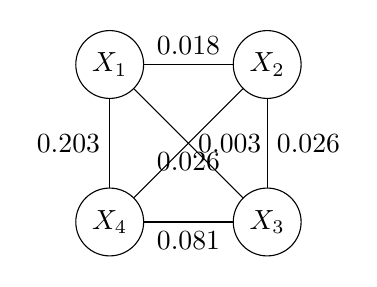
\begin{tikzpicture}
    % Nodes
    \node[circle, draw] (X1) at (0,2) {$X_1$};
    \node[circle, draw] (X2) at (2,2) {$X_2$};
    \node[circle, draw] (X3) at (2,0) {$X_3$};
    \node[circle, draw] (X4) at (0,0) {$X_4$};
    % Edges with weights
    \draw (X1) -- (X2) node[midway, above] {0.018};
    \draw (X1) -- (X3) node[midway, right] {0.003};
    \draw (X1) -- (X4) node[midway, left] {0.203};
    \draw (X2) -- (X3) node[midway, right] {0.026};
    \draw (X2) -- (X4) node[midway, below] {0.026};
    \draw (X3) -- (X4) node[midway, below] {0.081};
\end{tikzpicture}
\]

\item \textbf{Step 3: Finding the Maximum Spanning Tree}

We use Kruskal's algorithm to find the maximum spanning tree (MST) from the weighted graph, selecting edges that maximize the sum of mutual information while ensuring no cycles.

\textbf{Kruskal's Algorithm}:
\begin{enumerate}
    \item Sort edges by mutual information (descending order):
    \begin{itemize}
        \item \(X_1 - X_4\): 0.203
        \item \(X_3 - X_4\): 0.081
        \item \(X_2 - X_3\): 0.026
        \item \(X_2 - X_4\): 0.026
        \item \(X_1 - X_2\): 0.018
        \item \(X_1 - X_3\): 0.003
    \end{itemize}
    \item Initialize an empty tree.
    \item Add edges, skipping those that create cycles:
    \begin{itemize}
        \item Add \(X_1 - X_4\) (0.203): Connects \(X_1, X_4\), no cycle.
        \item Add \(X_3 - X_4\) (0.081): Connects \(X_3\) to \(X_4\), no cycle (\(X_1 - X_4 - X_3\)).
        \item Add \(X_2 - X_3\) (0.026): Connects \(X_2\) to \(X_3\), no cycle (\(X_1 - X_4 - X_3 - X_2\)).
        \item Skip \(X_2 - X_4\) (0.026): Creates cycle (\(X_2 - X_3 - X_4 - X_2\)).
        \item Skip \(X_1 - X_2\) (0.018): Creates cycle (\(X_1 - X_4 - X_3 - X_2 - X_1\)).
        \item Skip \(X_1 - X_3\) (0.003): Creates cycle (\(X_1 - X_4 - X_3 - X_1\)).
    \end{itemize}
    \item The tree has 3 edges, connecting all 4 nodes.
\end{enumerate}

\textbf{Maximum Spanning Tree}:
The MST includes edges:
\begin{itemize}
    \item \(X_1 - X_4\) (weight 0.203)
    \item \(X_3 - X_4\) (weight 0.081)
    \item \(X_2 - X_3\) (weight 0.026)
\end{itemize}
Total weight: \(0.203 + 0.081 + 0.026 \approx 0.310\).

\textbf{Visualization of the MST}:
\[
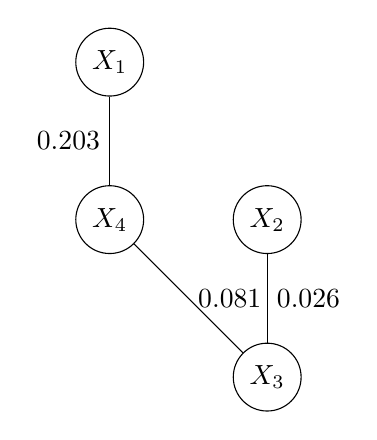
\begin{tikzpicture}
    % Nodes
    \node[circle, draw] (X1) at (0,2) {$X_1$};
    \node[circle, draw] (X2) at (2,0) {$X_2$};
    \node[circle, draw] (X3) at (2,-2) {$X_3$};
    \node[circle, draw] (X4) at (0,0) {$X_4$};
    % Edges with weights
    \draw (X1) -- (X4) node[midway, left] {0.203};
    \draw (X3) -- (X4) node[midway, right] {0.081};
    \draw (X2) -- (X3) node[midway, right] {0.026};
\end{tikzpicture}
\]




\end{enumerate}

\subsection{Scoring Function}
Using the BIC scoring metrics below, compute the model (graph and potentials) that generated the data below. 

\textbf{BIC:}
\[
S(G, \theta; D) = LL(\theta; D) - \phi(|D|)\|G\| \quad \text{where} \quad \phi(t) = \frac{\log(t)}{2}
\]

\textbf{Maximizing the score:}
\[
S_{\text{max}}(G, D) = \max_{\theta} \big(S(G, \theta; D)\big)
\]

\begin{figure}[H]
\centering
\includegraphics[width=0.8\textwidth]{q2.png}
\caption{The data used to compute the BIC score.}
\label{fig:data}
\end{figure}

\newpage
\section{Variational Inference}
\subsection{Mean-Field Approximation for Multivariate Gaussians}
In this question, we’ll explore how accurate a Mean-Field approximation can be for an underlying multivariate Gaussian distribution. Assume we have observed data \( X \in \mathbb{R}^{2 \times n} \) where each column \( X_{\cdot,i} \triangleq x^{(i)} \in \mathbb{R}^2 \) is a sample that was drawn from a 2-dimensional Gaussian distribution \( x^{(i)} \sim p(\cdot; \mu, \Lambda^{-1}) \).

\[
p(x; \mu, \Lambda) = \mathcal{N} \left( 
\begin{bmatrix}
x_1 \\
x_2
\end{bmatrix}
;
\begin{bmatrix}
\mu_1 \\
\mu_2
\end{bmatrix}
,
\begin{bmatrix}
\Lambda_{11} & \Lambda_{12} \\
\Lambda_{21} & \Lambda_{22}
\end{bmatrix}^{-1}
\right)
\tag{1}
\]

Note here that we’re using the precision matrix \( \Lambda = \Sigma^{-1} \). An additional property of the precision matrix is that it is symmetric, so \( \Lambda_{12} = \Lambda_{21} \). (This is a convenient simplifying assumption.) We will approximate this 2-dimensional Gaussian with a mean field approximation, \( q(x) = q(x_1)q(x_2) \), the product of two 1-dimensional distributions \( q(x_1) \) and \( q(x_2) \). For now, we won’t assume any form for these distributions.

\begin{enumerate}
    \item \textbf{Short Answer:} Write down the equation for \( \log p(X) \). (For this question, you can leave all of the parameters in terms of vectors and matrices, not their subcomponents.)
    \item \textbf{Short Answer:} Group together everything that involves \( X_1 \) and remove anything involving \( X_2 \). We claim that there exists some distribution \( q^*(X) = q^*(X_1)q^*(X_2) \) that minimizes the KL divergence \( q^* = \arg\min_q \text{KL}(q \| p) \). Furthermore, said distribution will have a component \( q^*(X_1) \) that will be proportional to the quantity you find below. Write that term that is proportional to \( q^*(X_1) \).
    \\\\ It can be shown that this implies that \( q(X_1) \) (and therefore \( q(X_2) \)) is a Gaussian distribution:
    \[
    q(x_1) = \mathcal{N} \left( x_1; m_1, \Lambda_{11}^{-1} \right)
    \]
    where 
    \[
    m_1 = \mu_1 - \Lambda_{11}^{-1} \Lambda_{12} \big(E[x_2] - \mu_2\big)
    \]
    Using these facts, we’d like to explore how well our approximation can model the underlying distribution.
    \item Suppose the parameters of the true distribution are 
    \[
    \mu = 
    \begin{bmatrix}
    0 \\
    0
    \end{bmatrix}
    \quad \text{and} \quad
    \Lambda = 
    \begin{bmatrix}
    1 & 0 \\
    0 & \frac{1}{4}
    \end{bmatrix}.
    \]
    
        \begin{enumerate}
            \item[(a)] \textbf{Numerical Answer:} What is the value of the mean of the Gaussian for \( q^*(X_1) \)?
            \item[(b)] (2 points) \textbf{Numerical Answer:} What is the value of the variance of the Gaussian for \( q^*(X_1) \)?
            \item[(c)] (2 points) \textbf{Numerical Answer:} What is the value of the mean of the Gaussian for \( q^*(X_2) \)?
            \item[(d)] (2 points) \textbf{Numerical Answer:} What is the value of the variance of the Gaussian for \( q^*(X_2) \)?
            \item[(e)] (5 points) \textbf{Plot:} Provide a computer-generated contour plot to show the result of our approximation \( q^*(X) \) and the true underlying Gaussian \( p(X; \mu, \Lambda) \) for the parameters given above.
        \end{enumerate}
    \item Suppose the parameters of the true distribution are 
    \[
    \mu = 
    \begin{bmatrix}
    1 \\
    2
    \end{bmatrix}
    \quad \text{and} \quad
    \Lambda = 
    \begin{bmatrix}
    \frac{2}{3} & -\frac{1}{3} \\
    -\frac{1}{3} & \frac{2}{3}
    \end{bmatrix}.
    \]
    
        \begin{enumerate}
            \item[(a)] (2 points) \textbf{Numerical Answer:} What is the value of the mean of the Gaussian for \( q^*(X_1) \)?
            \item[(b)] (2 points) \textbf{Numerical Answer:} What is the value of the variance of the Gaussian for \( q^*(X_1) \)?
            \item[(c)] (2 points) \textbf{Numerical Answer:} What is the value of the mean of the Gaussian for \( q^*(X_2) \)?
            \item[(d)] (2 points) \textbf{Numerical Answer:} What is the value of the variance of the Gaussian for \( q^*(X_2) \)?
            \item[(e)] (5 points) \textbf{Plot:} Provide a computer-generated contour plot to show the result of our approximation \( q^*(X) \) and the true underlying Gaussian \( p(X; \mu, \Lambda) \) for the parameters given above.
        \end{enumerate}
    \item (2 points) Describe in words how the plots you generated provide insight into the behavior of minimization of
    KL(q||p) with regards to the low probability and high probability regions of the true vs. approximate distributions.

    The contour plots illustrate the differences between the true distribution \( p(X; \mu, \Lambda) \) and the approximate distribution \( q^*(X) \). In high-probability regions, where the true distribution has significant density, the approximation \( q^*(X) \) closely aligns with \( p(X) \). This is because minimizing \( \text{KL}(q \| p) \) prioritizes matching the high-probability regions of \( p(X) \), as discrepancies in these regions contribute more to the KL divergence. Conversely, in low-probability regions, the approximation \( q^*(X) \) may deviate more significantly from \( p(X) \), as these regions have less influence on the overall KL divergence. This behavior reflects the trade-off inherent in the mean-field approximation, where the focus is on capturing the most probable regions of the true distribution while potentially sacrificing accuracy in less probable areas.
\end{enumerate}

\subsection{Variational Inference vs. Monte Carlo Methods}

Let’s end with a brief comparison between variational methods and MCMC methods. We have seen that both
classes of methods can be used for learning in scenarios involving latent variables, but both have their own sets of
advantages and disadvantages. For each of the following statements, specify whether they apply more suitably to
VI or MCMC methods:

\begin{enumerate}
    \item (2 points) Transforms inference into optimization problems.\\
    \(\bigcirc\) Variational Inference \(\checkmark\) \\
    \(\bigcirc\) MCMC
    \item (2 points) Is easier to integrate with back-propagation.\\
    \(\bigcirc\) Variational Inference \(\checkmark\) \\
    \(\bigcirc\) MCMC
    \item (2 points) Involves more stochasticity.\\
    \(\bigcirc\) Variational Inference \\
    \(\bigcirc\) MCMC \(\checkmark\)
    \item (2 points) Converges to the true distribution.\\
    \(\bigcirc\) Variational Inference \\
    \(\bigcirc\) MCMC \(\checkmark\)
    \item (2 points) Is higher variance under limited computational resources.\\
    \(\bigcirc\) Variational Inference  \\
    \(\bigcirc\) MCMC \(\checkmark\)
\end{enumerate}

\end{document}
